\documentclass[11pt,a4paper]{article}   % 11 pt text on A4 paper

% Page
\usepackage{csquotes}
\usepackage[backend=biber,style=apa,natbib=true]{biblatex} % APA 7; compile with Biber
\addbibresource{references.bib}

\usepackage[margin=2.5cm]{geometry}     % 2.5 cm margins all round
\usepackage{parskip}                    % a blank line between paragraphs instead of an indent

% Maths
\usepackage{amsmath}                    % align, cases, matrices and \text inside maths
\usepackage{mathtools}                  % fixes and extras for amsmath, such as \coloneqq
\usepackage{amssymb}                    % extra symbols such as \mathbb{R}
\usepackage{amsthm}                     % theorem, definition and proof environments

% Figures and tables
\usepackage{tikz}                       % drawing diagrams
\usepackage{pgfplots}                   % plotting functions and data, built on TikZ
\pgfplotsset{compat=1.18}               % use current pgfplots behaviour (label placement and so on)
\usepackage{tabularx}                   % tables that stretch to a set width

% Links
\usepackage[hidelinks]{hyperref}        % clickable cross-references, without coloured boxes
\hypersetup{                            % details shown in the PDF viewer’s document properties
  pdftitle  = {Week 4: Systems of linear differential equations},
  pdfauthor = {Your Name},
  pdflang   = {en-AU}
}

% Number equations, figures and tables by section: (2.1), Figure 2.1, ...
\numberwithin{equation}{section}
\numberwithin{figure}{section}
\numberwithin{table}{section}

% Theorem-like environments, all sharing one counter per section: Theorem 2.1, Example 2.2, ...
\theoremstyle{plain}                    % italic text, for statements
\newtheorem{theorem}{Theorem}[section]
\newtheorem{lemma}[theorem]{Lemma}
\newtheorem{corollary}[theorem]{Corollary}
\theoremstyle{definition}               % upright text, for definitions and examples
\newtheorem{definition}[theorem]{Definition}
\newtheorem{example}[theorem]{Example}
\theoremstyle{remark}                   % italic heading and upright text, for asides
\newtheorem{remark}[theorem]{Remark}
\newenvironment{solution}{\begin{proof}[Solution]}{\end{proof}}

\title{Week 4: Systems of linear differential equations}
\author{Your Name}
\date{Semester 2, 2026}

\begin{document}
\maketitle

\section{Eigenvalues and eigenvectors}

Throughout, $A$ is a real $2 \times 2$ matrix and $\mathbf{x}(t) \in \mathbb{R}^2$.

\begin{definition}
A number $\lambda$ is an \emph{eigenvalue} of $A$ if $A\mathbf{v} = \lambda\mathbf{v}$ for some
non-zero vector $\mathbf{v}$, called an \emph{eigenvector}. The eigenvalues are the roots of the
\emph{characteristic polynomial}
\begin{equation}\label{eq:char}
  p(\lambda) \coloneqq \det(A - \lambda I).
\end{equation}
\end{definition}

\begin{lemma}\label{lem:independent}
Eigenvectors $\mathbf{v}_1, \mathbf{v}_2$ belonging to distinct eigenvalues $\lambda_1 \neq \lambda_2$
are linearly independent.
\end{lemma}

\begin{proof}
Suppose $c_1\mathbf{v}_1 + c_2\mathbf{v}_2 = \mathbf{0}$. Applying $A - \lambda_2 I$ to both sides
gives $c_1(\lambda_1 - \lambda_2)\mathbf{v}_1 = \mathbf{0}$, so $c_1 = 0$, and then $c_2 = 0$.
\end{proof}

\section{Solving \texorpdfstring{$\mathbf{x}' = A\mathbf{x}$}{x' = Ax}}

\begin{theorem}\label{thm:general}
Suppose $A$ has distinct real eigenvalues $\lambda_1, \lambda_2$ with eigenvectors
$\mathbf{v}_1, \mathbf{v}_2$. Then every solution of $\mathbf{x}' = A\mathbf{x}$ has the form
\begin{equation}\label{eq:general}
  \mathbf{x}(t) = c_1 e^{\lambda_1 t}\mathbf{v}_1 + c_2 e^{\lambda_2 t}\mathbf{v}_2,
  \qquad c_1, c_2 \in \mathbb{R}.
\end{equation}
\end{theorem}

\begin{proof}
Each term solves the system, since
$\frac{d}{dt}\bigl(e^{\lambda t}\mathbf{v}\bigr) = \lambda e^{\lambda t}\mathbf{v}
= e^{\lambda t} A\mathbf{v} = A\bigl(e^{\lambda t}\mathbf{v}\bigr)$, and so does any linear
combination of them. By Lemma~\ref{lem:independent}, $\mathbf{v}_1$ and $\mathbf{v}_2$ form a basis, so we can
choose $c_1, c_2$ to match any initial value $\mathbf{x}(0)$, and by uniqueness of solutions
this is the only solution with that initial value.
\end{proof}

\begin{example}\label{ex:saddle}
Solve $\mathbf{x}' = A\mathbf{x}$ with
\[
  A = \begin{pmatrix} 1 & 2 \\ 2 & 1 \end{pmatrix}, \qquad
  \mathbf{x}(0) = \begin{pmatrix} 2 \\ 0 \end{pmatrix}.
\]
\end{example}

\begin{solution}
By \eqref{eq:char}, $p(\lambda) = (1 - \lambda)^2 - 4 = (\lambda - 3)(\lambda + 1)$, so the
eigenvalues are $\lambda_1 = 3$ and $\lambda_2 = -1$. Solving $(A - \lambda I)\mathbf{v} = \mathbf{0}$
gives
\[
  \mathbf{v}_1 = \begin{pmatrix} 1 \\ 1 \end{pmatrix}, \qquad
  \mathbf{v}_2 = \begin{pmatrix} 1 \\ -1 \end{pmatrix}.
\]
At $t = 0$, \eqref{eq:general} needs $c_1 + c_2 = 2$ and $c_1 - c_2 = 0$, so $c_1 = c_2 = 1$ and
\begin{align*}
  x_1(t) &= e^{3t} + e^{-t}, \\
  x_2(t) &= e^{3t} - e^{-t}.
\end{align*}
Figure~\ref{fig:phase} shows this trajectory in the phase plane.
\end{solution}

\begin{remark}
If the eigenvalues are complex, \eqref{eq:general} still holds with complex constants, and the real
and imaginary parts of $e^{\lambda_1 t}\mathbf{v}_1$ give two real solutions.
\end{remark}

\begin{figure}[ht]
  \centering
  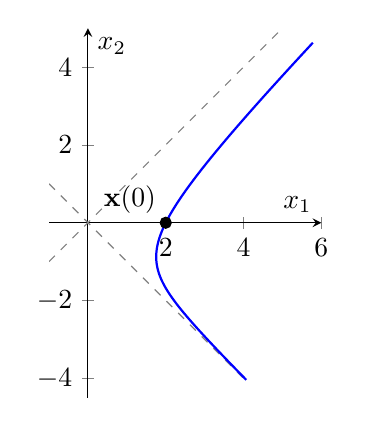
\begin{tikzpicture}
    \begin{axis}[
        width=0.6\textwidth, axis equal image, axis lines=middle,
        xmin=-1, xmax=6, ymin=-4.5, ymax=5,
        xlabel={$x_1$}, ylabel={$x_2$}]
      % the eigenvector directions
      \addplot[dashed, gray, domain=-1:6] {x};
      \addplot[dashed, gray, domain=-1:4] {-x};
      % the solution from the example, for t from -1.4 to 0.55
      \addplot[thick, blue, domain=-1.4:0.55, samples=100]
        ({exp(3*x) + exp(-x)}, {exp(3*x) - exp(-x)});
      \addplot[only marks, mark=*] coordinates {(2,0)} node[above left] {$\mathbf{x}(0)$};
    \end{axis}
  \end{tikzpicture}
  \caption{The solution of Example~\ref{ex:saddle} (blue) leaves along $\mathbf{v}_1$ as $t$ grows.
    The dashed lines are the eigenvector directions.}
  \label{fig:phase}
\end{figure}

\section{Summary}

The signs of the eigenvalues decide how solutions behave near the origin, as
Table~\ref{tab:cases} shows.

\begin{table}[ht]
  \centering
  \caption{Behaviour of $\mathbf{x}' = A\mathbf{x}$ by eigenvalue.}
  \label{tab:cases}
  \begin{tabularx}{0.85\textwidth}{l l X}
    \hline
    Eigenvalues & Origin & Behaviour of solutions \\
    \hline
    $\lambda_1, \lambda_2 < 0$ & stable node & every solution tends to $\mathbf{0}$ \\
    $\lambda_1, \lambda_2 > 0$ & unstable node & every non-zero solution grows without bound \\
    $\lambda_1 < 0 < \lambda_2$ & saddle & solutions come in along one eigenvector and leave along the other \\
    $\alpha \pm i\beta$, $\alpha, \beta \neq 0$ & spiral & solutions rotate, growing if $\alpha > 0$ and shrinking if $\alpha < 0$ \\
    $\pm i\beta$, $\beta \neq 0$ & centre & solutions circle the origin forever \\
    \hline
  \end{tabularx}
\end{table}

\printbibliography

\end{document}
